\documentclass[14pt]{article}
\usepackage[margin=0.8in]{geometry}
\usepackage{fancyvrb}
\usepackage{graphicx}
\usepackage{subcaption}
\usepackage{hyperref}
\hypersetup{
	colorlinks=true, %set true if you want colored links
	linkcolor=black, %choose some color if you want links to stand out
	urlcolor=blue
}
\graphicspath{ {./images/} }

\setlength{\parindent}{0pt}

\title{CCTF - Report}
\date{18/11/2020}
\author{Nail Dupre, Guadagnini Giovanni, Enrico Micheli, Davide Piva}

\begin{document}
	
\maketitle
	
\tableofcontents
\newpage
\section{Overview}
This report concern the two cctf laboratories:
\begin{itemize}
	\item \textbf{Resilient CCTF}: During this ctf the main purposes were both to attack and defend a HTTP server against different type of attacks.
	\item \textbf{Secure CCTF}: During this ctf the main purposes were both to attack and defend a small php webapp.
\end{itemize}

It's possible to find all the scripts and file used for this exercise in this \href{https://github.com/giovanniguadagnini/cctf-group5}{repository}.

\section{Resilient Server}
As already introduced in the Overview section this cctf was targeted to both offend and defend an HTTP server. Each group during the experience have access to two Deterlab experiments, in the first experiment the group will act as defenders (Blue Team) and in the second as attackers (Red Team).

\label{sec:TopologyExaplanation}
\begin{figure}[!h]
	\centering
	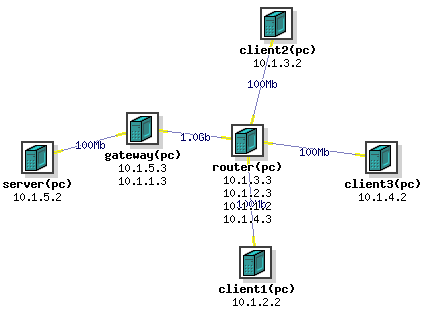
\includegraphics[width=8cm,height=6cm]{ResilientServerTopology}
	\caption{Topology of the Resilient Server CCTF.}
\end{figure}

This image describe the topology of the laboratory, that can be subdiveded in 3 areas:
\begin{itemize}
	\item \textbf{Clients machines}: These machines will be used from the attacker team. One of the three computer will be used as the genuine client that will try to reach the server with legitimate requests with a maximium rate of 1 request every second, the attackers will use the other two machines to attack the server in order to try to deny service to the genuine client.
	
	\item \textbf{Server and Gateway}: This two machine will be used from the defender team, in the specific the server will be equipped with a webserver, that serve 10 html pages, and the gateway will be used to try to block eventual attacks.
	
	\item \textbf{Router}: This machine will connect all the machines controlled from the two groups and will be used to calculate the score.
\end{itemize}

\textbf{Attention}: The link between router and gateway is different from all the other links. In the specific the link provide 1 gb of bandwidth and allows all the client connected to the router to send the maximum amount of data allowed from the 100 mb links, and this is very suitable to launch flood attacks.
\\
\\
During the ctf attackers earn a points when a genuine request from the client take more than 0.5 seconds to be received, and on the contrary the point is given to the defenders group if the request is received from the client before half a second is passed. 

\subsection{Dupre}

\subsection{Guadagnini}
The work started working by developing some milestones: 
\begin{itemize}
	\item monitor\_server.sh: This script perform a really fast check of the server status. By sending ping and curl requests the user can easily understand if the server it's slowed down by some attacks.
	
	\item analyze\_traffic.sh: This script launches two python programs that by using tcpdump, thanks to system function of os python module, and finally by analyzing the collected traffic, will enable the user to know with precision how many packets have passed through the gateway and also which client are sending data. This script in the end wasn't used since another version af the same script that uses only python seemed to be a bit faster.
	
	\item flood.sh: This is a simple script that act as a wrapper for the flooder program that will enable the user to flood an ip by specifying less parameter than usual.
	
	\item slow\_loris.py: This script has been dowloaded it from its repository and in the first moment has only been modified to request for the pages provided from the server.
\end{itemize}

The initial part has been concluded by writing the startup.sh script for all the machines involved the cctf:
\begin{itemize}
	\item Blue part startup.sh: This script by using ssh will connect to the server and will automatically install the apache2 webserver, enable syn-cookies, create the pages in the /var/html/www folder, enable the slow-loris mitigation for apache2, setup the iptable rules and finally upload the milestone scripts in a shared folder /home/cctf. Also will configure the gateway by uploading the script and configuring the iptables rules.
	
	\item Red part startup.sh: Through ssh will install all the packages needed and will all upload the milestone scripts on a shared folder /home/cctf in all the client machines.
\end{itemize}

In all the scripts the interface has been inserted as a parameter thanks to a sort of subscript that using the ip address of the interface was able to return the name of the interface as a result.
\begin{Verbatim}
# Retrieve the name of the internal interface of the gateway machine
$(ip a | grep 10.1.5.3 | tail -c 5)
\end{Verbatim}

\subsubsection{Strategy}
Has also been developed the defense and attack strategy, that which over time have been modified according to the results obtained during the internal tests.

\paragraph{Defense strategy}
The first idea used was to limit the attack surface to a minimum and therefore to reduce it to a minimum and indispensable, so the iptables both on server and gateway have been used to try to block the unnecessary traffic. A white list approach has been used to allow only some kind of traffic to pass and finally reach the server, in the specific has been allowed:
\begin{itemize}
	\item All the traffic from loopback interface.
	\item All the traffic generated and directed to deterlab control network (192.168.0.0/16).
	\item All icmp traffic between gateway and server in the network 10.1.5.0/24.
	\item Icmp packet generated from the external network with a maximum rate of 1 ICMP packet per second.
	\item The fragmented packets have been blocked to avoid fragmented attacks.
	\item All the incoming http traffic on port 80, and obviously the outgoing traffic generated from the server.
\end{itemize}
Finally has been specified the DROP default policy for all the iptables chains in order to block all the traffic that won't match the rules. 
\\
Rules configured in the gateway:
\begin{Verbatim}
sudo iptables -F
sudo iptables -A INPUT -i lo -j ACCEPT
sudo iptables -A OUTPUT -o lo -j ACCEPT
sudo iptables -A INPUT -s 192.168.0.0/16 -j ACCEPT
sudo iptables -A OUTPUT -d 192.168.0.0/16 -j ACCEPT
sudo iptables -A FORWARD -f -j DROP
sudo iptables -A FORWARD -p tcp -d 10.1.5.2 -s 10.1.2.0/24,10.1.3.0/24,10.1.4.0/24 --dport 80 
	-m state --state NEW,ESTABLISHED -j ACCEPT
sudo iptables -A FORWARD -p tcp -s 10.1.5.2 -d 10.1.2.0/24,10.1.3.0/24,10.1.4.0/24 --sport 80 
	-m state --state ESTABLISHED -j ACCEPT
sudo iptables -A INPUT -f -j DROP
sudo iptables -A INPUT -p icmp --icmp-type echo-request -s 10.1.5.2 
	-i \$(ip a | grep 10.1.5.3 | tail -c 5) -j ACCEPT
sudo iptables -A OUTPUT -p icmp --icmp-type echo-reply 
	-o \$(ip a | grep 10.1.5.3 | tail -c 5) -d 10.1.5.2 -j ACCEPT
sudo iptables -A OUTPUT -p icmp --icmp-type echo-request -o $(ip a | grep 10.1.5.3 | tail -c 5) 
	-d 10.1.5.2 -j ACCEPT
sudo iptables -A INPUT -p icmp --icmp-type echo-reply -i $(ip a | grep 10.1.5.3 | tail -c 5) 
	-s 10.1.5.2 -j ACCEPT
sudo iptables -A OUTPUT -p tcp --dport 80 -d 10.1.5.2 -o $(ip a | grep 10.1.5.3 | tail -c 5) -j ACCEPT
sudo iptables -A INPUT -p tcp --sport 80 -s 10.1.5.2 -i $(ip a | grep 10.1.5.3 | tail -c 5) -j ACCEPT
sudo iptables -A INPUT -i $(ip a | grep 10.1.1.3 | tail -c 5) -d 10.1.1.3 
	-s 10.1.2.0/24,10.1.3.0/24,10.1.4.0/24 -p icmp --icmp-type echo-request 
		-m hashlimit --hashlimit-name icmp_gw --hashlimit-mode srcip 
			--hashlimit 1/second --hashlimit-burst 5 -j ACCEPT
sudo iptables -A OUTPUT -o $(ip a | grep 10.1.1.3 | tail -c 5) -s 10.1.1.3 
	-d 10.1.2.0/24,10.1.3.0/24,10.1.4.0/24 -p icmp --icmp-type echo-reply 
		-m hashlimit --hashlimit-name icmp_gw --hashlimit-mode srcip 
			--hashlimit 1/second --hashlimit-burst 5 -j ACCEPT
sudo iptables -A FORWARD -i $(ip a | grep 10.1.1.3 | tail -c 5) 
	-d 10.1.5.2 -s 10.1.2.0/24,10.1.3.0/24,10.1.4.0/24 -p icmp 
		-m hashlimit --hashlimit-name icmp_srv --hashlimit-mode srcip 
			--hashlimit 1/second --hashlimit-burst 5 --icmp-type echo-request -j ACCEPT
sudo iptables -A FORWARD -o $(ip a | grep 10.1.1.3 | tail -c 5) -s 10.1.5.2 
	-d 10.1.2.0/24,10.1.3.0/24,10.1.4.0/24 -p icmp 
		-m hashlimit --hashlimit-name icmp_srv --hashlimit-mode srcip 
			--hashlimit 1/second --hashlimit-burst 5 --icmp-type echo-reply -j ACCEPT
sudo iptables -P INPUT DROP
sudo iptables -P OUTPUT DROP
sudo iptables -P FORWARD DROP
\end{Verbatim}

To protect the server against slow DoS attacks, such as slow-loris, the libapache2-mod-qos has been enabled and configured, this module basically disables the keep-alive messages when the connections in the pool are running out in order to try to keep the service online and available.
\\
\\ 
Moreover, in an attempt to reduce problems related to malicious opening of connections with the web server, the apache timeout time has been reduced from 300 seconds to 1 second which for the purpose of this competition is sufficient to keep a connection active for the time used to assign a point.
\\
\\
\textbf{Snort} was also tried to improve defenses with some basic rules. By using the installation script present in the an older laboratory in the end Snort was installed in the gateway. Snort in particular can be very useful for thwarting some attacks but it is very harmful for flooding attacks as being single thread it does not scale very well when the number of requests rises significantly. So using Snort was very useful since was able to stop slow\_loris attack very easily but when a simple Syn flood attack was initiated, the performance collapsed causing significant delays in delivering the packets to the server and therefore to the genuine client. another problem with snort was the installation time, in fact before using the program it was necessary to wait for snort to compile and install on the system which took a long time. For the reasons outlined above snort was discarded and other techniques were sought and subsequently used.
\\
\\
As a result of the attacks tested, the security measures implemented were able to defend the server from slow dos attack thanks to the apache module but were vulnerable to flood attacks as a way to limit large amounts of traffic directed to the server had not yet been implemented.
\\
\\
From the beginning rate limiters used with Snort or iptables seemed not suitable since they were cutting off good and malicious traffic without distinction for a certain amount of time. The final idea for the defense was trying to inspect the traffic and search difference between genuine and malicious traffic, in order to let only packets that should be genuine through the gateway. Two very useful iptables option has been found and used to cut the malicious traffic. In the specific the two modules named named \textbf{match-hex} and \textbf{match-string} by inspecting the content of the packets were able to identify malicious packets. 
\\
So in the end the defense, in addition to some configurations made in the server, consisted of 2 steps:
\begin{itemize}
	\item Use tcpdump and Wireshark to collect data and search for differences or special pattern in the packets.
	\item Use the two iptables modules to cut the traffic identified as malicious during the previous step.
\end{itemize}

Despite the large traffic generated by flood attacks, iptables, with a limited number of rules used to filter incoming traffic, has always managed to maintain good performance and for this reason it has been used as the main part of the defense.

\paragraph{Attack strategy}
Defense and attack strategies were developed simultaneously, when a problem was solved a new attack that took advantage of more sophisticated methods was created and used to try to send the server out of service. This process of continuos modifications led to the modification of the attacks so that with each "iteration" each attack was better and in the specific each time the attack were modified in order that it had been more difficult to distinguish genuine from malicious traffic. 
\\
\\
In an attempt to optimize the score gained / lost during the attack phase, the following idea was formulated and used: if the attacks we were using weren't working or were partially working, there was no need to send the maximum requests possible and accordingly to this fact the genuine traffic could be lowered to the minimum or just simply reduced to lower the number of points opponents were earning. So following this idea the genuine\_client.sh script was modified to change on-demand the rate of the request sent by reading a file created in the same folder, the rate could be easily modified using the script change\_rate.sh that remotely throug ssh was able to modify the rate value saved on the file.
\\
\\
In order for the slow\_loris.py to be less recognizable, the request header has been redefined to be the same of curl and the content of the keep-alive requests has been randomized in order to be more difficult to detect and block. 
\\
\\
By observing the attacks has been suggested also to use scripts or packages that were able to modify the header fields in order to make the attack packes as indistinguishable as possible from genuine traffic, for example by putting the window at the same value that is used by curl 64240 and using modified headers as for the slow loris attack.
\\
\\
Finally has been discovered that while using flood attacks a single process wasn't able to generate very big amount of traffic, for example over 70000 packet per second. So accordingly to the available bandwidth of the link has been suggested to lower down the number of packets generated from a single process during flood attacks in order to make sure to take advantage of the available bandwidth with multiple processes that were concurrently generating a reasonable number of packets.

\subsubsection{Results Evaluation}
During the two cctfs by analyzing the traffic an by using the match module of iptables the defenses were able to cut a very big amount of malicious traffic. 
\\
\\
During the first cctf, before the laboratory crashed a very big portion of the attack traffic was blocked from the gateway and it seemed that the server was able to respond to genuine requests quickly.
\\
\\
Unfortunately in the second ctf the adversary team has been were very smart and managed to make the defenses to be ultra-protective. In fact, using fragmented genuine requests, which were blocked by default by the gateway, they managed to score many points as the requests to the server never arrived. One of the methods used to defend, in addition to blocking fragmented packets, was in fact to check that the DF (do not fragment) bit was not set to 1 in requests, this was typical in syn packets of flood attacks, but unfortunately it was also used from the other team to generate the genuine requests. Also by interspersing fragmented and non fragmanted genuine requests they managed to "protect" their attack as it seemed that the server was working correctly.

\begin{figure}[!h]
	\centering
	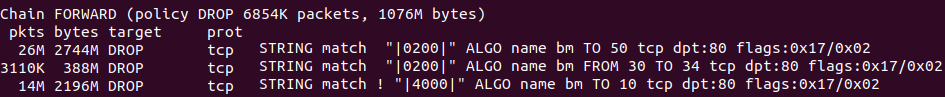
\includegraphics[width=20cm,height=1.5cm]{iptables_cctf_1}
	\caption{FORWARD iptables chain in gateway cctf1.}
\end{figure}

\begin{figure}[!h]
	\centering
	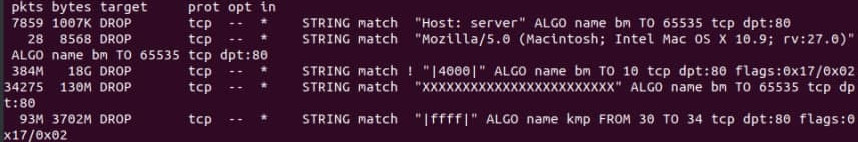
\includegraphics[width=20cm,height=3cm]{iptables_cctf_2}
	\caption{FORWARD iptables chain in gateway cctf2.}
\end{figure}
This images shows the rules added during the two cctf, as it's possible to see from the second column, the amount of dropped traffic is very big aroung 25 GB if we consider both the cctf. 
\\
In the specific the rules used were similar to the following:
\begin{Verbatim}
# Check for window = 65535
sudo iptables -I FORWARD 1 --match string --algo bm --from 30 --to 34 --hex-string '|ff ff|' 
-p tcp --dport 80 --syn --j DROP 

# Check for DF bit not setted typical of flooder
sudo iptables -I FORWARD 1 --match string --algo bm --to 10 ! --hex-string '|4000|' 
-p  tcp --dport 80 --syn --j DROP 

# Check for syn packet with malicious string in the playload
sudo iptables -I FORWARD 1 --match string --string "<malicious_content>" 
-p tcp --dport 80 --syn --j DROP
\end{Verbatim}

Has been really useful also the option "to" and "from" of the match iptables module since 
they could help narrow down which portion of the package to look for the pattern or malicious content.

\subsection{Micheli}

\subsection{Piva}

\section{Secure Server}
During this second ctf the objectives were to defend and attack a small web application. The modality of the exercise are the same used during the first ctf and the topology is the same, the only difference is in the fact that within this competition syn flood attacks are not allowed.
\\
As already stated topology and machines involved are the same as in the Resilient ctf to refresh the concepts take a look to the overview of the \hyperref[sec:TopologyExaplanation]{Resilient Server}. 
\\
\\
During this ctf, the point were earned as red team when sending malicious request the red team was able to create inconsistency in the defender database, on the contrary the blue team earned points if they managed to deny the creation of incosistencies in the database. 

\subsection{Dupre}

\subsection{Guadagnini}
For this ctf the work started by developing fixing the process.php script code, of which all the decisions regarding fixes are illustrated in the next paragraph, continued with the development of the stratup.sh scritps, that to be fair the script are more or less the same used for the resilient ctf, there are only slight modifications related to the fact that this time the used packages are different:
\begin{itemize}
	\item Blue startup.sh: Is automatically configuring the iptables of gateway and server machine to accept traffic directed to server port 80, eventual ping traffic limited to 1 operation per second from all the network of the laboratory and it's blocking all the other traffic. To conclude the script has been modified to install LAMPP, apply the patch agains slow loris attacks, fix the database problem by running an .sql file and finally by loading all the script in /home/cctf folder.
	
	\item Red startup.sh: This script is installing all the needed packages and uploading all the attack script on /home/cctf folder.
\end{itemize} 

Finally the work ended by developing the missing milestones:
\begin{itemize}
	\item check\_consistency\_db.sh: This script is really useful to check if the attackers are creating problems to the database integrity, in the specific two queries are executed in order to spot if some users has a negative balance and also if some transactions exists for users non registered in the system, all these two contidions should be ensured from the patches applied to the php script but also from the foreign key constraint that has been added to the database. In any case it's a good pratice to check that these conditions are always in place since the adversary may have some new attacks that could not be fixed from the used implementation. During the ctf this script has been modified to monitor the number of users and transactions generated.
	
	\item connect\_to\_client.sh: This script by exploiting port forwarding capabilities of deterlab and a proxy tunnel between the client and a browser allowed the user to connect to the adversary server using one of the clients connected tho the deterlab experiment, really useful to test some attacks.
	
	\item genuine\_request.sh: This script is really simple and after performing the registration of the user in the system it keeps sending deposit and withdraw operations 
	interspersed with one second waits, to generate genuine traffic to the adversary server.
	
	\item basic\_attack.sh: This script tries to exploit the fact the adversary process.php is not pathced against slow operations. The idea is really simple and it's subdivided in two parts:
	\begin{enumerate}
		\item The script using the same account used for the genuine\_request.sh keep running deposit and withdraw operations.
		\item When some time passed and the user has a lot of transactions, the script was launched to keep requesting for balance while the genuine\_request.sh keep doing it's work. In this way the server should slow down and some consistency problem may be generated from the high workload.
	\end{enumerate} 
	It very simple to see if the php script wasn't patched and was only needed to request for a balance page after the genuine\_request.sh script was running for a while, if the page was really big than the attack may be possible.
	
	\item attack.py: This is also a very simple attack script that using a predefined list of payloads that may generate problems to the adversary implmentation. Specifically, the script tries to create malicious requests by inserting payloads in the various combinations of valid and non-valid requests that are generated and sent to the server, after sending the request, before proceeding with the next try, the script shows the result code and the returned page in order for the user to evaluate if the attack was successful or not.
\end{itemize}

\subsubsection{Strategy}
As happened for the resilient ctf a strategy has been created and optimized as result of all the work done and also from the analysis of the services involved in the laboratory. In the specific, for the defense phase all the vulnerabilities identified in the php has been mitigated and also some iptables rule has been employed in both server and gateway to regulate the traffic that was able to reach the server; instead for the attack phase some really general attacks that tries to exploit the fixed vulnerabilities has been created.

\paragraph{Defense phase}
For the defense, the work started by applying the patch needed to secure the php script:
\begin{itemize}
	\item \textbf{SQL injections}: The first problem fixed was relative to sql injection, in the specific the application wasn't performing any type of checks on the data before executing the query, this is really unsecure since an attacker could exploit this security problem to run whatever command he wants to run in our database and this can bring problem like data leaks and incosistencies. So in order to fix this problem prepared statement has been implemented in all the query that used parameter, as for the next small example script:
	\begin{Verbatim}[tabsize=4]
	$stm = $mysqli->prepare("INSERT INTO transfers (user,amount) values (?, ?)");
	$stm->bind_param("si", $user, $amount);
	if ($stm->execute() == false){
		closeDBandFile($stm->error); // In case of error print the error 
			//and close the connection with files and mysql 
	}
	\end{Verbatim}
	Applying prepare statements the webapp is secure against this kind of attack.
	
	\item \textbf{Possible XSS}: Also it was almost immediately noticed the possibility to create problems to the user exploiting the fact that on 'user' and 'pass' field of the request no checks were performed, so it was really simple to use them to execute XSS injections. This problem was fixed using \textbf{htmlentites} function of php that in escape all the characters and make impossible for an attacker to exploit this issue.
	
	\item \textbf{Credential checks and security}: The original implementation of the process.php script wasn't checking the user credentials before executing the operations, so it was possible for an attacker to perform operations also for users that weren't present in the system. To fix this problem an authentication function has been added and used to protect the execution of malicious requests.
	\begin{Verbatim}
	if ($choice == 'register') {
		...
	} else if ($choice == 'balance' && checkUserCredentials($user, $pass) == true) {
		...
	} else if ($choice == 'deposit' && checkUserCredentials($user, $pass) == true) {
		...
	} else if ($choice == 'withdraw' && checkUserCredentials($user, $pass) == true) {
		... 
	} 
	\end{Verbatim}
	So after the fix was possible to perform balance, deposit and withdraw, that implicitly consider that the user is present in the system, only if the user credentials provided has been verified, obviously in order to avoid useless work to the database the function that verify the user credentials is called only if the user setted all the parameter in a correct and managed to get to the operation without problems.
	\\
	The second problem with the password was that in the database the password were stored in clear so possible data leak could be very dangerous for the registered users also no checks on the minumum password lenght were enforced. To fix this problem the code has beed updated to user \textbf{password\_hash} and \textbf{password\_verify} php functions and a simple check on the paramter has been added to check that the password was at least 10 characters long, in this way the user need to insert a password that is at least 10 characters long and the password are stored in the database hashed to reduce the risks. A function that checks if the password is secure could also been interesting to add to the script to enhance the security level of the password. 
	\begin{Verbatim}[tabsize=4]
	...
	//user registration
	$stm = $mysqli->prepare("INSERT INTO users (user, pass) VALUES (?, ?)");
	$stm->bind_param("ss", $user, password_hash($pass, PASSWORD_DEFAULT)); // The password is stored 
		//in the database as the digest generated from the php function
	...
	/*
	* Check the user credential, in the specific retrieve the digest of the password and checks
	* it with password_verify function
	* $user Username of the user we need to check the credentials
	* $pass Password inserted
	* return outcome of the password digest check
	*/
	function checkUserCredentials($user, $pass){
		$stm = $GLOBALS['mysqli']->prepare("SELECT pass FROM users WHERE user = ?");
		$stm->bind_param("s", $user);
		
		if ($stm->execute() == false){
			closeDBandFile($stm->error); // In case of error print the error 
				//and close the connection with files and mysql 
		}
		
		$result = $stm->get_result();
		$row = $result->fetch_array();
		if(!password_verify($pass, $row['pass'])){ // Password is check using 
			//the digest verification funciton of php
			closeDBandFile("User doesn't exist in the system or the combination "+
				"user and password used is wrong, retry!");
			return false;
		}
		
		return true;
	}	
	\end{Verbatim}
	Finally for the user present in the system the password has been randomly generated and updated in the database accordingly to the new specifics.
	
	\item \textbf{Parameters check}: As already stated all the parmeter in the original version of the script were using without perform any check at all. To fix this problem some checks has been implemented especially in two point of the code:
	\begin{enumerate}
		\item At the beginning of the code some checks has been implemented to ensure the user inserted all the parameters in the request and also it was checked that the username could be stored in the user field of the database. In case the parameter that is missing is really important, like for example username or password, the execution is blocked and a message is sent to the user.
		
		\item The second part of this checks was related to the amount parameter, in the specific the script is checking the number inserted is an integer with the \textbf{intval} php function, that converts string to integers, and also checks if it's within the limit of the database integer type. All this checks and cast operations are applied to ensure there are no problem on the execution of the query and also to provide precise error messages to the users.
	\end{enumerate}

	\item \textbf{Problem on withdraw operation}: In the original script it was possible to create incosistencies in the database since it wasn't performing checks on the amount of money during the withdraw operations. This problem was fixed by getting from the database the amount of money of a user and by checking if the user could withdraw the amount of money inserted.
	\begin{Verbatim}[tabsize=4]
	/*
	* Get the user balance from the database
	* $user Username of the user we need to recover the balance
	* return balance of the user
	*/
	function getUserBalance($user){
		$stm = $GLOBALS['mysqli']->prepare("SELECT SUM(amount) 
			as amount FROM transfers where user = ? ");
		$stm->bind_param("s", $user);
		
		if ($stm->execute() == false){
			closeDBandFile($stm->error); // In case of error print the error 
				//and close the connection with files and mysql 
		}
		
		$result = $stm->get_result(); // Retrieve the information from the database
		$row = $result->fetch_array();
		$amount = $row['amount'];  
		
		// If the result set is empty than set the amount to 0
		if(!$amount){
			$amount = 0;
		}
	
		return $amount;
	}
	\end{Verbatim}
	About the deposit, since the database is able to sum the integer and if needed automatically performs the cast to a bigger type in case the result is to big for the used type, there is no need to check if the user amount is bigger than the integer type of the database, the only limit is regarding the transactions amount that need to be within the mysql integer type limits. 
	
	\item \textbf{Slow operations}: It was immediately clear that some operations with the database were very slow and could be used against the web application. In the specific two slow operations are executed when the balance operation is specified from the user and are the balance calculation and the transfers history visualization. To solve this problem two things has been added:
	\begin{itemize}
		\item The balance has been calculated using a sql query, this is faster than getting all the results from the database and calculate the balance by summing all the rows in case the transfers are a lot, also the database should mantain good performances also if in the table are present a lot of rows. In the specific every time the balance of the user is needed the \textbf{getUserBalance} function is used.
		
		\item The second problem has been fixed by limiting the data that a single page can visualize by implementing a simple pagination of the results, in the specific the user is limited to view 25 results per page and can easily navigate through the transactions using a navigation bar. In this way even if the user has thousands of transactions the performance should remain good, and the server should answer in short amount of time also during high workloads.
	\end{itemize}
	
	\item \textbf{Database problems}: Finally the database has been fixed the problems found were related to how the database tables were created and from the user used from the php script. In the specific the first problem was that the relation between the two tables wasn't enforced, so it was possible to insert transfers of users not registered, also by inserting the foreign key constraint the engine used (MyISAM) wasn't checking the foreign key, the second problem related to the user is that the php script using the root user can access to all the tables present in the system and perform everything since all the operations are allowed to that user this is a very big problem if for some reason an attacker is able to exploit a vulnerability and use the db user at his will.
	The problem has been solved by:
	\begin{itemize}
		\item The table engine has been modified to InnoDB that is able to enforce foreign key constraint and finally a foreign key constraint has been added to ensure the transaction belong to an existing user.
		
		\item The principle of least privileges has been enforced to evaluate the operations needed from the php script and an user has been created accordingly. In the specific the user can only access to the ctf2 database and only SELECT and INSERT operations are allowed.
	\end{itemize}
	\begin{Verbatim}
	CREATE USER 'php_user'@'localhost' IDENTIFIED BY '|AttackersWontFindOut@';
	GRANT SELECT ON ctf2.users TO 'php_user'@'localhost';
	GRANT SELECT ON ctf2.transfers TO 'php_user'@'localhost';
	GRANT INSERT ON ctf2.users TO 'php_user'@'localhost';
	GRANT INSERT ON ctf2.transfers TO 'php_user'@'localhost';
	ALTER TABLE ctf2.users MODIFY COLUMN pass char(64) NOT NULL;
	ALTER TABLE ctf2.users ENGINE = InnoDB;
	ALTER TABLE ctf2.transfers ENGINE = InnoDB;
	ALTER TABLE ctf2.transfers ADD CONSTRAINT users_transfers_fk FOREIGN KEY (user)
		REFERENCES ctf2.users(user);
	\end{Verbatim}
	
	\item \textbf{File and database connection}: Thanks to Piva intuition the application after the fix automatically closes the stream with the file and the connection with the database, this is really important since during the normal usage of the php script the page will be executed concurrently from many users and since the resource are limited is a good practice to release them in a correct way to allow other process to use them.
	
	\item \textbf{Log}: Since the log original implementation was logging all the evantual parameters the user insert in the request, has been added into the php script a small section of the log part that in order to evaluate the attacks was logging only the parameter used from the php script in the specific name, surname, drop and amount.
	
	\item \textbf{Other fix}: Finally the application has been completed by arranging eventual error message and a very minimal style for the page.
\end{itemize}

To continue the defense evaluation, even if some services won't be available because of the iptables rules that will be configured in the machines, a research on the vulnerability of the used software has been performed. These are the results:
\begin{itemize}
	\item \textbf{Apache 2.4.29}: The top 5 known vulnerabilities has a CVSSv4 score smaller than 7.3 and basically seems to be related to some modules that are configured and used from the attacker in order to try to stop the server, but since apache is being used with a very simple configuration it seems that no known vulnerability can be used to affect server. \href{https://www.cvedetails.com/vulnerability-list.php?vendor_id=45&product_id=66&version_id=241078&page=1&hasexp=0&opdos=0&opec=0&opov=0&opcsrf=0&opgpriv=0&opsqli=0&opxss=0&opdirt=0&opmemc=0&ophttprs=0&opbyp=0&opfileinc=0&opginf=0&cvssscoremin=0&cvssscoremax=0&year=0&month=0&cweid=0&order=3&trc=18&sha=e3f39e55231940b8282f47396e556881d5954cd3}{List of known vulnerabilies}.
	
	\item \textbf{Php 7.2.24}: Generally there are a lot of known vulnerabilities (34) for the version 7.x of php, but seems that all the vulnerability are patched before the version used from LAMPP. \href{https://www.cvedetails.com/vulnerability-list.php?vendor_id=74&product_id=128&version_id=235668&page=1&hasexp=0&opdos=0&opec=0&opov=0&opcsrf=0&opgpriv=0&opsqli=0&opxss=0&opdirt=0&opmemc=0&ophttprs=0&opbyp=0&opfileinc=0&opginf=0&cvssscoremin=0&cvssscoremax=0&year=0&month=0&cweid=0&order=3&trc=34&sha=2f75abb453af67c2cfdd59ab77666b9572304c78}{List of known vulnerabilies}.
	
	\item \textbf{Mysql 5.7.31}: The result are practically the same obtained while analyzing php known vulnerabilities. Also, we should be safe, by considering that the mysql server isn't directly accessible from outside the server, so for an eventual attacker should be very difficult to gain access to this component of the system to exploit vulerabilities. \href{https://www.cvedetails.com/vulnerability-list.php?vendor_id=93&product_id=21801&version_id=242149&page=1&hasexp=0&opdos=0&opec=0&opov=0&opcsrf=0&opgpriv=0&opsqli=0&opxss=0&opdirt=0&opmemc=0&ophttprs=0&opbyp=0&opfileinc=0&opginf=0&cvssscoremin=0&cvssscoremax=0&year=0&month=0&cweid=0&order=3&trc=100&sha=620313f8a90c589726af95aa0b4d06477f2a7496
	}{List of known vulnerabilies}.
\end{itemize}

Finally to complete the analysis some test with a network fuzzer has been performed. In the specific \href{https://github.com/xmendez/wfuzz}{wfuzz} has been used and by using apache.txt and sql\_inj.txt wordlist some test has been performed to ensure the implemented security measures were strong enough. 
\begin{verbatim}
wfuzz -c -w /home/giovanni/Scaricati/wfuzz/wordlist/vulns/apache.txt 
	"http://localhost:8080/process.php?user=FUZZ&pass=FUZZ&amount=FUZZ&drop=FUZZ"

wfuzz -c -w /home/giovanni/Scaricati/wfuzz/wordlist/vulns/apache.txt 
	"http://localhost:8080/process.php?user=test1&pass=test1test1test1&amount=FUZZ&drop=deposit"

wfuzz -c -w /home/giovanni/Scaricati/wfuzz/wordlist/vulns/apache.txt 
	"http://localhost:8080/process.php?user=test1&pass=test1test1test1&amount=FUZZ&drop=withdraw"
\end{verbatim}
These are some of the command that has been executed to test the security of the php script, all the test performed gave negative results and the application seemed to answer well.
It's possible to find more information on the recon phase in the files contained in the repo.
\\
\\
A possible use of Snort was evaluated but finally discarded since the protection provided by the iptables rules and its match-string module allowed to effectively protect the webapp

\paragraph{Attack phase}
As happened for the resilient ctf the attacks has been created trying to exploit vulnerabilities found in the original implementation, for this reason attack script as basic\_attack.sh and attack.py has been created. To be fair it was difficult to create original attacks that deviate from exploiting slow operations or sql injections and it was also very difficult to exploit volumetric attacks increasing the number of requests since basically we were allowed to send 1 request per second from each client. It was also difficult to create other exploit because the used software seemed to be secure against known vulnerabilities and if the traffic was well managed from the adversary firewall was really difficult to reach the machines and eventual vulnerable services.

\subsubsection{Results Evaluation}
As for the first ctf I personally enjoyed the experience, overall during the ctf the implemented defense held up really good to the received attacks in fact from the monitoring software I dind't noticed consistency problem and the server seemed to be up and fast for all the duration ctf. I noticed the adversary tried to run a really basic version of slow loris that I blocked with an iptables rules since the keep-alive messages contained a recongnizable string. I also noticed they tried to exploit remote code execution with a remote shellcode that didn't worked and also they tried with sqlinjection. Most of the time they tried to create users in the system in fact they managed to create more than 60000 users. 

\begin{figure}[h!]
	\centering
	\begin{subfigure}[b]{0.35\linewidth}
		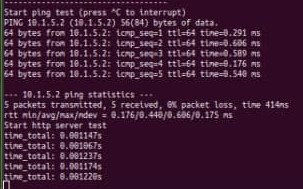
\includegraphics[width=\linewidth]{server_response_time}
		\caption{Server response time from monitoring software.}
	\end{subfigure}
	\begin{subfigure}[b]{0.3\linewidth}
		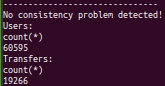
\includegraphics[width=\linewidth]{db_status}
		\caption{Database status from monitoring software.}
	\end{subfigure}
	\caption{These two images represent the system status at the end of the ctf.}
\end{figure}

To be fair after 1 hour and half our disk was full because the log file reached 11GB of dimension, this seemed to be my fault since in the process.php script I was using the same file for the normal logs and also the original version of the log but also seems to ba a consequence of the adversary red team script tha was generating to much traffic, the monitoring software detected 1955 packet in 5 seconds and I think the very high number of request ended up in creating a very big log file.
\begin{figure}[!h]
	\centering
	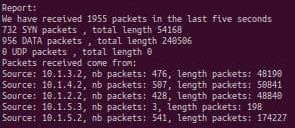
\includegraphics[width=6cm,height=3cm]{dos_ctf_secure}
	\caption{Traffic data collected in 5 seconds.}
\end{figure}

In retrospect I think that in addition to the applied changes I would have implemented, as suggested during the debriefing, a sort of filter to limit the creation of malicious users by checking for the presence of special characters or something similar also I would have liked to have snort with some rules to detect some attacks. 
\\
\\
As far as the attack phase is concerned, our attacks have not had a great effect, and what has created problems for the opposing blue team seems to have been an incorrect configuration.

\subsection{Micheli}

\subsection{Piva}

\end{document}
